\chapter{Literature Survey}

\section{Foundations of Grammatical Error Correction}

\subsection{Definition and Scope of GEC}

Grammatical Error Correction (GEC) is a subfield of Natural Language Processing (NLP) concerned with automatically transforming erroneous sentences into grammatically acceptable forms while preserving intended meaning \cite{ng-etal-2014-conll}. Although traditionally focused on morpho-syntactic violations such as subject--verb agreement, tense errors, article misuse, and word order \cite{bryant-etal-2017-automatic}, contemporary systems address a broader range of deviations, including spelling, punctuation, lexical choice, and limited sentence restructuring \cite{10.1162/coli_a_00478}. In practice, GEC therefore extends beyond narrow rule enforcement to improving clarity and overall comprehensibility.

The literature commonly distinguishes between \textit{grammaticality}, \textit{fluency}, and \textit{style} \cite{napoles-etal-2017-jfleg}. Grammaticality concerns conformity to linguistic rules, fluency refers to naturalness and readability, and style reflects authorial preference rather than correctness. Modern neural systems increasingly optimise for fluency, often producing broader rewrites rather than minimal edits \cite{loem2023exploringeffectivenessgpt3grammatical}. This creates a practical difficulty for GEC: a sentence may sound better after correction while also moving away from the learner's own wording. The distinction between grammatical correction and writing enhancement therefore matters for both evaluation and learner feedback \cite{ke2019automated}.

This distinction is especially important in learner-facing GEC, where a polished sentence is not always the most useful form of feedback. A system can improve fluency while reducing the visibility of the original grammatical error, so benchmark accuracy and pedagogical usefulness should not be treated as identical.

\subsection{Historical Evolution of GEC Systems}

GEC has developed alongside wider changes in NLP, moving from rule-based systems to statistical models and, more recently, large-scale neural architectures \cite{10.1162/coli_a_00478}.

\subsubsection{Rule-Based Systems}

Early GEC systems relied on hand-crafted linguistic rules designed to detect and correct specific error types. These systems typically targeted well-defined morpho-syntactic phenomena, such as subject--verb agreement, article usage, and verb tense errors \cite{ng-etal-2014-conll}. Rule-based approaches offered interpretability and precise control over corrections, but they were limited by coverage. Building and maintaining large rule sets required linguistic expertise, and such systems struggled when learner errors fell outside predefined categories \cite{10.1162/coli_a_00478}.

\subsubsection{Statistical Machine Translation (SMT)-Based GEC}

Statistical Machine Translation (SMT) changed the way GEC was framed. Rather than treating correction as isolated rule application, SMT-based approaches treated it as a monolingual translation task, converting ``incorrect'' sentences into corrected counterparts \cite{brockett2006correcting}. This allowed systems to learn correction patterns from parallel corpora of learner text and annotated revisions.

SMT approaches improved flexibility and coverage compared to rule-based systems \cite{ng-etal-2014-conll}. However, they remained dependent on aligned training data and often required complex feature engineering. They were also not explicitly designed to preserve minimal edits, so broader sentence-level changes could still appear in the output \cite{10.1162/coli_a_00478}. This is an early example of the tension between correction accuracy and minimality.

\subsubsection{Neural Sequence-to-Sequence Models}

With the emergence of neural sequence-to-sequence (Seq2Seq) architectures \cite{NIPS2014_5a18e133}, GEC systems began to benefit from distributed representations and end-to-end learning. Neural models, particularly those incorporating attention mechanisms \cite{bahdanau2016neuralmachinetranslationjointly}, improved fluency and contextual coherence in corrected outputs. Unlike SMT systems, neural approaches required less manual feature engineering and were better able to model long-range dependencies within sentences.

Neural Machine Translation (NMT) approaches became dominant in shared tasks, outperforming SMT systems on benchmarks such as CoNLL-2014 and subsequent evaluations \cite{ng-etal-2014-conll,10.1162/coli_a_00478}. However, increased fluency introduced a new problem: neural models could prefer natural-sounding output even when a smaller grammatical edit would be enough. This raised concerns about over-correction and unnecessary rewriting, particularly in educational contexts \cite{napoles-etal-2017-jfleg}.

\subsubsection{Transformer-Based Approaches}

The introduction of Transformer architectures \cite{NIPS2017_3f5ee243} further advanced GEC performance. Transformer-based models use self-attention to capture relationships between words across a sentence, making it easier to represent wider context and connections between distant parts of the text. These models achieved state-of-the-art results on shared tasks and benchmarks, establishing neural architectures as the dominant paradigm in GEC \cite{bryant-etal-2019-bea}.

At the same time, the generative capacity of Transformer-based systems increased the likelihood of sentence rewriting rather than targeted correction. As models became more fluent and context-aware, the distinction between grammatical correction and broader rewriting became progressively less clear. This development set the stage for the emergence of LLMs, which extend Transformer architectures to unprecedented scale and capability \cite{NEURIPS2020_1457c0d6}.

\begin{figure}[h]
    \centering
    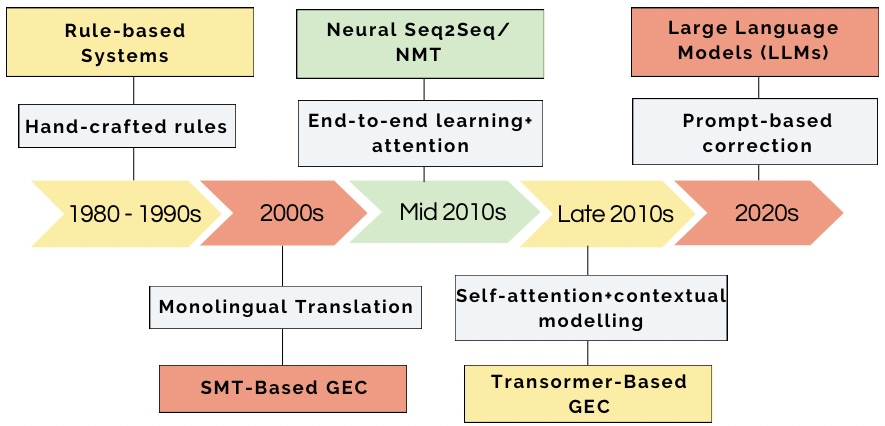
\includegraphics[width=13cm]{figures/evolution_of_gec.PNG}
    \caption{Evolution of Grammatical Error Correction Approaches}
    \label{fig:gec-timeline}
\end{figure}

\section{Large Language Models in GEC}

Large Language Models (LLMs) extend Transformer-based approaches by using broad linguistic knowledge acquired through large-scale pre-training. In GEC, this allows correction behaviour to be elicited through prompts rather than task-specific retraining. This shift is important for the present study because prompt wording becomes a key factor in determining whether the model performs minimal correction or broader rewriting.

\subsection{From Fine-Tuned Models to Prompt-Based GEC}

Traditional neural GEC systems relied on supervised fine-tuning using annotated learner corpora such as NUCLE and W\&I + LOCNESS \cite{ng-etal-2014-conll,bryant-etal-2019-bea}. These systems were optimised for edit-based metrics such as $F_{0.5}$, and their performance depended on the size and coverage of available annotated datasets.

Large Transformer-based models, including GPT-3 \cite{NEURIPS2020_1457c0d6}, showed that autoregressive language models can perform new tasks through in-context learning. In this setting, the model responds to instructions and optional examples in the prompt without updating its internal parameters.

For GEC, this makes zero-shot and few-shot correction possible. Zero-shot prompting provides only task instructions, such as ``Correct grammatical errors'', while few-shot prompting includes example input--output pairs that demonstrate the desired correction behaviour \cite{NEURIPS2020_1457c0d6}. Empirical studies show that LLMs can achieve competitive correction performance under these conditions despite the absence of task-specific training \cite{loem2023exploringeffectivenessgpt3grammatical}.

However, prompt-based GEC differs from supervised encoder--decoder systems. Because LLMs are trained to generate fluent and plausible continuations rather than to minimise edits, their outputs are influenced by instruction phrasing and contextual framing. Prompt design therefore becomes an important mechanism for influencing correction scope and over-correction risk.

This also means that high-quality LLM output can be ambiguous from an evaluation perspective: the same fluency that makes a correction readable may also conceal unnecessary rewriting. The present study therefore treats fluency as a useful signal, but not as sufficient evidence that a correction is pedagogically appropriate.

\subsection{Advantages of LLM-Based GEC}

LLM-based GEC offers advantages in fluency, generalisation, and adaptability.

First, LLMs are able to produce well-formed and contextually coherent corrections because they are pre-trained on large and diverse text corpora using next-token prediction objectives \cite{NEURIPS2020_1457c0d6}. Empirical studies report that GPT-style models can correct surface-level grammatical errors while also improving naturalness and readability \cite{loem2023exploringeffectivenessgpt3grammatical}.

Second, LLMs are less dependent on task-specific annotated corpora. Unlike fine-tuned systems trained on datasets such as NUCLE or W\&I + LOCNESS, LLMs can apply linguistic knowledge from broad pre-training to correction tasks through prompting alone \cite{ng-etal-2014-conll,bryant-etal-2019-bea,NEURIPS2020_1457c0d6}. This makes them more flexible across domains and may help with error types that are underrepresented in benchmark datasets.

Third, prompt-based interaction allows correction behaviour to be adjusted without retraining. Changes in instruction wording, role framing, or examples can influence the scope of the correction \cite{liu2023pretrain}. This adaptability is useful for exploring minimal-edit correction strategies, although it also introduces variability in model behaviour.

\subsection{Known Weaknesses of LLM-Based GEC}

The same generative properties that make LLMs useful for GEC also create limitations. Three concerns are especially relevant to this dissertation: hallucination, over-editing, and prompt instability.

Hallucination refers to the introduction of content that is not present or implied in the input sentence \cite{maynez2020faithfulness}. In GEC, this may involve semantic additions, altered meaning, or unnecessary clarification. Even small meaning shifts can be problematic because correction should preserve the learner's intended message.

Over-editing occurs when the model rephrases or restructures a sentence beyond what is needed for grammatical correction \cite{loem2023exploringeffectivenessgpt3grammatical}. Although this can improve readability, it may reduce minimality and transparency, especially in educational contexts where learners need to understand what was corrected and why. This issue is examined in more detail in Section~\ref{sec:over-correction}.

Prompt instability refers to the sensitivity of model outputs to changes in instruction wording or example selection \cite{liu2023pretrain}. Carefully engineered prompts may encourage more restrained corrections, but they do not guarantee consistent behaviour. For this reason, the present study compares prompt-induced variation empirically rather than assuming that a constraint in the prompt will always be followed.

\subsection*{Summary}

LLMs make GEC more flexible by enabling correction through prompting rather than task-specific fine-tuning. They offer strong fluency, broad generalisation, and adaptable control through prompt design. However, their generative nature also creates risks, including hallucination, over-editing, and prompt instability. These risks motivate the next section, which examines fluency bias, over-correction, and their implications for learner-facing GEC.

\section{Over-Correction and Educational Alignment}
\label{sec:over-correction}

LLM-based GEC systems can produce fluent and natural-sounding corrections, but this strength can also lead to over-correction. In this dissertation, over-correction refers to cases where the model changes the learner's wording, vocabulary, or sentence structure beyond what is needed for grammatical repair, especially when those changes do not provide clear benefit.

One reason for this behaviour is fluency bias. Because LLMs are trained to generate probable and natural-sounding text, they may favour polished sentences over minimal edits \cite{NEURIPS2020_1457c0d6,NIPS2017_3f5ee243}. In GEC, this can appear as lexical substitution, clause restructuring, or broader rephrasing. Although these changes may improve readability, they can also move the correction away from the learner's original expression \cite{loem2023exploringeffectivenessgpt3grammatical}.

Over-correction is difficult to define as simply incorrect, because some broader revisions may be useful in context. However, in learner-facing GEC, excessive rewriting can reduce the pedagogical value of feedback. Minimal correction allows learners to compare the original and corrected forms more directly, supporting noticing and reflection \cite{schmidt1990role}. By contrast, fluency-oriented rewriting may introduce several changes at once, making it harder to identify the specific source of the error.

This creates an alignment issue. The intended goal of educational GEC is targeted grammatical repair with minimal necessary modification, while the learned behaviour of LLMs often favours fluent sequence generation. As a result, a model may produce an output that is grammatically acceptable but less useful as feedback for L2 learners.

\subsection{Illustrative Example}

\begin{figure}[h]
    \centering
    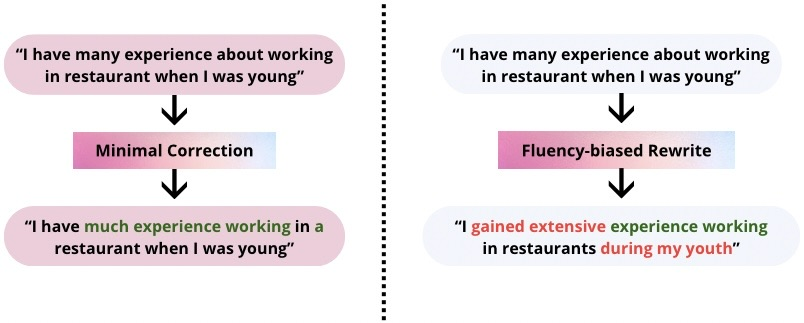
\includegraphics[width=13cm]{figures/minimal_vs_fluency.PNG}
    \caption{Minimal Correction vs Fluency-biased Rewrite}
    \label{fig:minimal-vs-fluency}
\end{figure}

The minimal correction changes only the grammar that needs correction, while keeping the structure of the learner's sentence largely intact. The fluency-biased rewrite introduces lexical substitution and structural reformulation. This increases the amount of modification and makes the original error less visible.

\subsubsection*{Comparative Summary}
\begin{table}[htbp]
\centering
\caption{Pedagogical Comparison: Minimal Correction vs Fluency-Biased Rewrite}
\label{tab:pedagogical_comparison}
\begin{tabular}{|p{4cm}|p{4cm}|p{5cm}|}
\hline
\textbf{Dimension} & \textbf{Minimal Correction} & \textbf{Fluency-Biased Rewrite} \\
\hline
Edit Scope & Localised changes & Structural reformulation \\
\hline
Learner Wording & Preserved & Modified \\
\hline
Error Transparency & High & Reduced \\
\hline
Support for Noticing & Facilitates comparison & May obscure error locus \\
\hline
Dependency Risk & Lower & Higher \\
\hline
\end{tabular}
\end{table}

These differences show why over-correction cannot be understood through grammatical accuracy alone. To evaluate learner-facing GEC systems more appropriately, it is necessary to consider grammatical validity alongside the extent and usefulness of changes made to the learner's original sentence. The next section therefore reviews existing GEC evaluation metrics and their limitations for measuring unnecessary rewriting.

\section{Evaluation in GEC: Metrics and Limitations}

Having discussed over-correction in LLM-based GEC, this section reviews how correction quality is evaluated. Standard GEC evaluation usually focuses on grammatical accuracy by comparing system outputs with human reference corrections. This is useful for measuring whether a system corrects grammatical errors, but it does not fully show whether the system has changed the learner's original wording more than necessary. For this reason, learner-facing GEC requires both accuracy-based evaluation and source-output analysis.

\subsection{ERRANT and the M\textsuperscript{2} Scorer}

Standard GEC evaluation is usually based on comparison with human-annotated reference corrections. One widely used metric is the M\textsuperscript{2} (MaxMatch) scorer, introduced by Dahlmeier and Ng \cite{dahlmeier-ng-2012-better}. M\textsuperscript{2} evaluates system outputs by aligning proposed edits with gold-standard edits and calculating an F-score over the matched edits. It was used as the official evaluation metric for the CoNLL-2014 shared task \cite{ng-etal-2014-conll}.

M\textsuperscript{2} is edit-based rather than sentence-based. It extracts edits from a system output and measures how many of these edits match the annotated correction. Performance is usually reported using precision, recall, and $F_{0.5}$.

\paragraph{Precision.}
Precision measures the proportion of system edits that are correct:
\[
\text{Precision} = \frac{\text{Correct Edits}}{\text{System Edits}}
\]
High precision means that the system's proposed edits are usually valid.

\paragraph{Recall.}
Recall measures the proportion of gold edits that the system successfully identifies:
\[
\text{Recall} = \frac{\text{Correct Edits}}{\text{Gold Edits}}
\]
High recall means that the system captures a larger share of the errors in the reference correction.

\paragraph{$F_{0.5}$ Score.}
In GEC, $F_{0.5}$ is commonly reported because it gives more weight to precision than recall:
\[
F_{0.5} =
\frac{(1 + 0.5^2)\cdot \text{Precision} \cdot \text{Recall}}
{0.5^2 \cdot \text{Precision} + \text{Recall}}
\]
This weighting reflects the importance of avoiding false positives, since unnecessary edits can reduce correction quality \cite{ng-etal-2014-conll}.

ERRANT extends this edit-based approach by automatically aligning the original learner sentence with the corrected sentence and assigning edits to linguistic error categories \cite{bryant-etal-2017-automatic}. This makes it useful for analysing grammatical correction quality in a more interpretable way. ERRANT can therefore show not only whether a correction matches the reference, but also what type of grammatical edit has been made.

However, ERRANT and M\textsuperscript{2} remain primarily accuracy-based metrics. They reward agreement with annotated edits, but they do not directly measure whether a system has rewritten the learner's sentence more than necessary.

This limitation matters because unnecessary rewriting may appear as a fluent alternative rather than an obvious error. As a result, a system can look strong under edit-alignment metrics while still producing feedback that is less transparent for a learner.

\subsection{Limitations of Accuracy-Only Evaluation}

Accuracy-based metrics are useful for benchmarking GEC systems, but they are limited when the correction can be expressed in several valid ways. A system output may be grammatically acceptable but receive a lower score if it does not match the available reference annotation. Conversely, an output may align with a reference correction while still making additional lexical or structural changes.

This issue becomes more important for LLM-based GEC because LLMs can produce fluent outputs that go beyond minimal grammatical repair. Fluency-oriented datasets such as JFLEG \cite{napoles-etal-2017-jfleg} show that correction can involve wider revision, while studies of GPT-style systems report similar tendencies towards rewriting \cite{loem2023exploringeffectivenessgpt3grammatical}.

For learner-facing GEC, this creates a mismatch between grammatical accuracy and pedagogical usefulness. A correction may improve surface fluency but make the learner's original error less visible. Evaluation therefore needs to consider not only whether the correction is accurate, but also how much the output changes and whether those changes are useful.

The gap is not that ERRANT or M\textsuperscript{2} are unsuitable for GEC; they remain valuable for measuring reference-based correction accuracy. Rather, they need to be complemented by source-output measures when the research question concerns over-correction risk and preservation of learner wording.

\subsection{Measuring Textual Change and Minimality}

To analyse over-correction risk, the corrected output can be compared directly with the original learner sentence. This source-output perspective captures aspects of correction behaviour that reference-based accuracy metrics do not measure.

Several types of measures can support this analysis. Word-level edit distance measures surface rewriting, while edit density adjusts this change by sentence length. Lexical diversity and readability measures can indicate shifts in vocabulary and sentence complexity. Similarity-based measures can estimate whether the corrected output remains close to the source sentence in meaning and form.

However, the amount of change should not be interpreted in isolation. Some corrections may alter the original sentence while still preserving meaning and improving fluency. For this reason, over-correction risk should be interpreted through both the extent of change and the apparent usefulness of that change.

\subsubsection{Edit Distance and Minimality}

Levenshtein distance \cite{levenshtein1966binary} compares two strings by identifying the minimum number of insertions, deletions, or substitutions needed to transform one into the other. In GEC, word-level edit distance can provide a direct indication of how much the model output differs from the learner sentence. Lower edit distance suggests a more minimal correction, while higher edit distance suggests broader rewriting.

However, edit distance alone cannot determine whether an edit is necessary. A sentence with several grammatical errors may require multiple changes, while a fluent but unnecessary rewrite may also produce a high edit distance. For this reason, edit distance is best understood as one signal of textual change rather than as a complete measure of over-correction.

\subsubsection{BLEU and SARI}

Other metrics, such as BLEU and SARI, are relevant to the wider discussion of text revision, although they are not sufficient for measuring over-correction in this study. BLEU \cite{papineni2002bleu} measures n-gram overlap between a system output and one or more reference corrections. Although it is widely used in machine translation, it does not directly capture minimality. A heavily rewritten sentence may still receive reasonable overlap with a reference, while a valid alternative correction may be penalised for using different wording.

SARI \cite{xu2016optimizing}, originally developed for text simplification, evaluates additions, deletions, and retained words. It is conceptually relevant because it rewards appropriate retention of the original sentence. However, SARI was designed for simplification rather than grammatical correction, so it is treated here as background rather than as the main evaluation metric.

\subsubsection{Structural and Lexical Change Indicators}

Beyond edit distance, structural and lexical indicators can help capture broader forms of rewriting. Type--Token Ratio (TTR) can be used to observe changes in lexical diversity, while readability measures such as the Flesch--Kincaid Grade Level \cite{kincaid1975derivation} can indicate changes in sentence complexity. Cosine similarity over lexical or syntactic features can also provide an estimate of similarity between the original and corrected sentence \cite{koppel2009computational}.

These measures do not judge grammatical correctness directly. Their purpose is to indicate how far the output has moved away from the learner's original sentence. They are therefore useful as complementary signals when analysing whether a correction preserves the learner's wording or rewrites it more substantially.

\subsection{Worked Example}

Consider:
\begin{figure}[h]
    \centering
    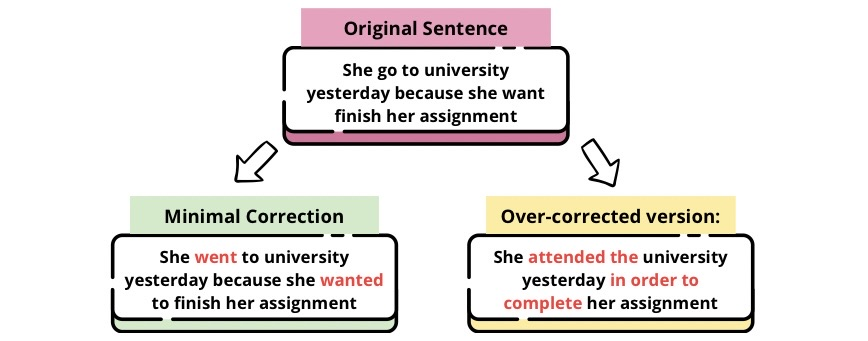
\includegraphics[width=\textwidth]{figures/minimal_vs_overcorrection.PNG}
    \caption{Minimal vs Over-Corrected Sentence}
    \label{fig:gec-example}
\end{figure}

The minimal correction introduces only necessary grammatical changes. Word-level edit distance remains low, and the structure of the learner sentence is mostly preserved.

In contrast, the over-corrected version replaces several lexical items, such as ``went'' with ``attended'', ``because'' with ``in order to'', and ``finish'' with ``complete''. It also changes the phrasing more broadly. These changes increase edit distance, affect readability and lexical properties, and reduce similarity to the original sentence.

This example shows why grammatical correctness alone is not enough to distinguish minimal correction from unnecessary rewriting. A fuller evaluation of learner-facing GEC therefore needs to consider both correction accuracy and the extent and usefulness of changes made to the original sentence.

\subsection{Comparative Summary of Metrics}

\begin{table}[h]
\centering
\caption{Comparison of Evaluation Metrics for GEC and Textual Change}
\label{tab:metric_comparison}
\begin{tabular}{|p{3cm}|p{5cm}|p{6cm}|}
\hline
\textbf{Metric} & \textbf{Measures} & \textbf{Limitation in GEC Context} \\
\hline
M\textsuperscript{2} / ERRANT & Edit alignment accuracy & Does not directly measure unnecessary rewriting \\
\hline
Levenshtein Distance & Magnitude of surface change & Cannot distinguish necessary from unnecessary edits \\
\hline
BLEU & N-gram overlap & Penalises valid alternatives; insensitive to minimality \\
\hline
SARI & Add/Delete/Keep operations & Designed for simplification, not grammar correction \\
\hline
TTR & Lexical diversity change & Sensitive to sentence length \\
\hline
Flesch--Kincaid & Readability change & Indirect proxy for structural modification \\
\hline
Cosine similarity & Source-output similarity & Does not identify grammatical correctness \\
\hline
\end{tabular}
\end{table}

Traditional edit-based metrics remain useful for measuring grammatical accuracy, but they are not sufficient for analysing over-correction risk. This motivates the evaluation strategy used in later chapters, where ERRANT-based accuracy is considered alongside change-based and utility-sensitive measures of rewriting behaviour.

\section{Prompt Engineering as Behavioural Control}

Given the limitations of accuracy-only evaluation and the risk of over-correction, prompt engineering becomes a practical way to influence how LLMs perform GEC without task-specific fine-tuning. In this dissertation, prompt design is treated as a form of behavioural control because it shapes how the model interprets the correction task and how far it is likely to move from the learner's original wording.

Prompt engineering refers to the design of instructions, roles, and examples that guide model outputs without changing the model's internal parameters \cite{liu2023pretrain}. Unlike supervised fine-tuning, which updates model weights, prompting works through input conditioning \cite{NEURIPS2020_1457c0d6}. In GEC, this means that the prompt can influence whether the model performs minimal grammatical repair or produces a broader rewrite.

\subsection{Prompting Strategies for Behavioural Control}

The prompting strategies considered in this dissertation can be grouped into three main types: instruction-constrained prompts, role-based prompts, and few-shot prompts. These strategies differ in how they guide the model. Instruction-constrained prompts define the task and limit the correction scope, role-based prompts frame the model's stance, and few-shot prompts demonstrate the desired correction behaviour through examples.

\subsubsection{Instruction-Constrained Prompts}

Instruction-constrained prompting uses explicit natural-language instructions to define both what the model should do and what it should avoid. In zero-shot settings, the model receives only the instruction and the input sentence, without demonstration examples \cite{NEURIPS2020_1457c0d6}. The wording of the instruction is therefore important.

For example, a generic prompt such as:

\begin{quote}
``Correct the following sentence.''
\end{quote}

leaves the correction scope open. The model may interpret ``correct'' as including grammar, fluency, vocabulary improvement, and sentence rewriting. This can lead to changes beyond what is needed for grammatical repair.

A more constrained instruction, such as:

\begin{quote}
``Correct only grammatical errors. Do not change word choice or sentence structure unless strictly necessary.''
\end{quote}

attempts to narrow the scope of correction and align the output with minimal-edit principles. Research on instruction tuning and prompting shows that LLMs are sensitive to task framing and that explicit constraints can influence output characteristics \cite{wei2022finetuned,liu2023pretrain}. However, these constraints are not strict rules. Because LLMs remain generative systems, they may not follow the instruction consistently in every case. Overly restrictive instructions may also prevent legitimate corrections when some restructuring is grammatically necessary.

\subsubsection{Role-Based Prompts}

Role-based prompting guides the model by assigning it a specific role or perspective. For example:

\begin{quote}
``You are an English teacher providing minimal grammatical corrections to an L2 learner.''
\end{quote}

This framing may encourage the model to behave less like a general editor and more like a teacher giving targeted feedback. Role conditioning has been shown to influence tone, lexical choices, and interpretive stance in LLMs \cite{wei2022finetuned,liu2023pretrain}. In GEC, an educational role may therefore support more restrained correction and better alignment with learner needs.

However, role-based prompts are also indirect. Their effects depend on associations learned during pre-training, so they may be less predictable than explicit constraints. A role prompt may encourage minimal correction, but it cannot guarantee that the model will avoid broader rewriting.

\subsubsection{Few-Shot and Example-Driven Prompts}

Few-shot prompting provides demonstration examples within the prompt \cite{NEURIPS2020_1457c0d6}. Instead of relying only on an instruction, the model is shown input--output pairs that illustrate the expected correction style. In GEC, these examples can demonstrate minimal-edit behaviour directly.

Few-shot examples can be powerful because they show the model what kind of transformation is expected. Prior work on in-context learning suggests that examples can shape model behaviour, sometimes more strongly than abstract instructions alone \cite{liu2023pretrain}. However, example-driven prompts also require careful design. Poorly chosen examples may encourage repeated rewriting patterns, while longer prompts increase computational cost and may approach context-length limits.

\subsection{Prompt Sensitivity and Control Limits}

Although prompting provides a practical way to guide LLM behaviour, it does not provide complete control. Prompt fragility refers to the way model outputs can change when a prompt is reworded, even if the intended task remains the same \cite{liu2023pretrain}. In GEC, a small change from ``correct grammatical errors'' to ``improve the sentence'' may shift the output from targeted repair towards broader rewriting.

This sensitivity occurs because in-context learning changes model behaviour through conditioning rather than parameter updates \cite{NEURIPS2020_1457c0d6}. Prompts therefore act as soft steering mechanisms rather than fixed rules. They can influence correction behaviour, but they do not guarantee that the output will always follow the intended correction strategy.

This creates an alignment challenge for learner-facing GEC. The intended goal is minimal grammatical correction, but the model may still favour fluent and polished output because it has been trained to generate natural-sounding text. For educational use, correction behaviour therefore needs to be evaluated, not simply assumed from the prompt wording.

\subsection{Synthesis and Research Focus}

The prompting strategies discussed above provide different ways to influence correction behaviour. Instruction-constrained prompts place explicit limits on editing, role-based prompts frame the model as a pedagogical assistant, and few-shot prompts demonstrate minimal correction through examples. All three strategies may help reduce unnecessary rewriting, but their effectiveness is uncertain because prompt adherence is not guaranteed.

This dissertation therefore asks a focused empirical question: whether a small set of structured prompting strategies can reduce over-correction risk relative to a simple baseline prompt while maintaining broadly comparable grammatical correction performance in an L2-focused setting.

\subsubsection*{Conceptual Control Framework}

In zero-shot and few-shot settings, the main controllable element is the prompt. The learner sentence remains the same, and the model parameters are not updated. Figure~\ref{fig:prompt_pipeline} shows where prompt specification sits in the correction pipeline.

\begin{figure}[htbp]
\centering
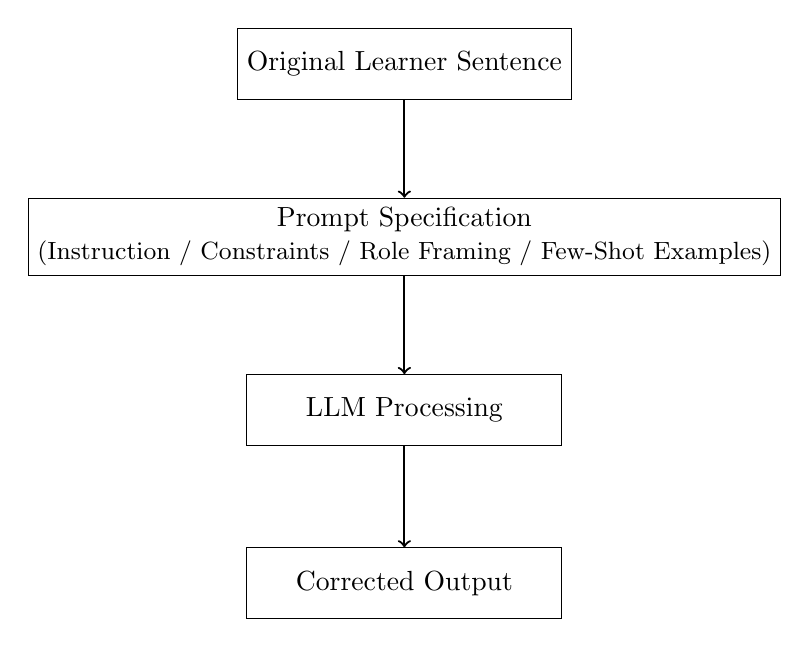
\begin{tikzpicture}[
node distance=2.2cm,
every node/.style={draw, rectangle, align=center, minimum width=4cm, minimum height=0.9cm}
]
\node (input) {Original Learner Sentence};
\node (prompt) [below of=input] {Prompt Specification \\ \small (Instruction / Constraints / Role Framing /
Few-Shot Examples)};
\node (model) [below of=prompt] {LLM Processing};
\node (output) [below of=model] {Corrected Output};

\draw[->, thick] (input) -- (prompt);
\draw[->, thick] (prompt) -- (model);
\draw[->, thick] (model) -- (output);

\end{tikzpicture}
\caption{Conceptual control points in prompt-based grammatical error correction}
\label{fig:prompt_pipeline}
\end{figure}

This framework motivates the experimental design used in later chapters, where structured prompts are tested to examine whether they can improve grammatical accuracy while reducing unnecessary rewriting.

\section{Ethical and Professional Considerations}

Using LLM-based GEC tools in education raises issues beyond technical performance. Because these systems can move from grammatical correction into broader rewriting, they affect learner agency, transparency, fairness, privacy, and academic integrity.

\subsection{Human--AI Interaction, Transparency, and Learner Agency}

LLM-based writing systems may generate fully revised sentences rather than targeted corrections. This can shift agency away from the learner, especially when the system performs revision on the learner's behalf instead of supporting self-correction.

Human--AI interaction research emphasises that AI systems should augment, rather than replace, human cognitive effort \cite{amershi2019guidelines}. In educational contexts, feedback is most useful when learners can understand the correction and use it for revision. Studies of automated writing evaluation show that learner uptake depends on clarity, perceived fairness, and opportunities for iterative improvement \cite{ke2019automated}. Overly broad or opaque corrections may therefore reduce reflective engagement.

Transparency is also important. A system is more transparent when learners can see what has been changed and understand why. Earlier rule-based systems often linked corrections to identifiable grammatical rules, whereas LLMs generate corrections through less interpretable statistical representations \cite{NIPS2017_3f5ee243}. Prompting can influence correction scope, but it does not automatically provide explanations. Without highlighted edits or rationales, learners may struggle to identify the grammatical issue. This connects with wider responsible AI principles, including transparency, accountability, and user awareness in high-impact domains such as education \cite{floridi2018ai4people}.

\subsection{Risk Analysis}

Integrating LLM-based correction tools into L2 learning environments introduces several risks.

\subsubsection{Learner Dependency and Reduced Critical Engagement}

If a system provides fully rewritten sentences, learners may rely on automated revision rather than engaging with their own errors. This may reduce learner autonomy and weaken metalinguistic awareness \cite{ke2019automated}. It may also limit the noticing process, where conscious attention to linguistic form supports acquisition \cite{schmidt1990role}. For this reason, feedback should support comparison and reflection rather than simply replace the learner's revision effort.

\subsubsection{Linguistic Homogenisation and Bias}

LLMs are trained on large-scale text corpora that reflect dominant linguistic norms. Their corrections may therefore standardise learner writing towards particular registers or dialects \cite{NEURIPS2020_1457c0d6}. In multicultural educational settings, unnecessary rewriting may reduce legitimate variation in expression. Fairness requires distinguishing genuine grammatical errors from acceptable linguistic variation \cite{floridi2018ai4people}.

\subsubsection{Data Privacy and Security}

Processing learner writing raises privacy concerns, particularly when texts include personal or sensitive information. This project uses an existing anonymised corpus and does not collect new participant data, so the practical risk is lower than in a deployed classroom system. Even so, secure storage, limited retention, and careful handling of model inputs remain important safeguards.

\subsubsection{Academic Integrity and Misuse}

Minimal grammatical correction differs from content generation, but the boundary between editing and rewriting can become blurred. Without clear usage guidelines, AI-assisted correction tools may affect authorship transparency, especially in assessment contexts.

\subsubsection*{Structured Risk Assessment}

Table~\ref{tab:risk_assessment} summarises the principal risks and corresponding mitigation strategies.

\begin{table}[htbp]
\centering
\caption{Risk Assessment for LLM-Based Grammatical Error Correction}
\label{tab:risk_assessment}
\begin{tabular}{|p{4cm}|p{3cm}|p{3cm}|p{4cm}|}
\hline
\textbf{Risk} & \textbf{Likelihood} & \textbf{Impact} & \textbf{Mitigation Strategy} \\
\hline
Learner Dependency & Medium & High & Emphasise minimal correction; encourage revision comparison \\
\hline
Reduced Critical Engagement & Medium & High & Provide highlighted edits; integrate explanatory feedback \\
\hline
Linguistic Homogenisation & Medium & Medium & Limit unnecessary rewriting and preserve learner wording where possible \\
\hline
Data Privacy Breach & Low--Medium & High & Anonymise data; limit storage; ensure regulatory compliance \\
\hline
Academic Misuse & Medium & High & Establish clear usage guidelines; distinguish correction from generation \\
\hline
\end{tabular}
\end{table}

\subsection{Study Safeguards}

This study uses anonymised learner data and does not collect additional personal information. The experiments store only the source sentences, prompt labels, model outputs, and evaluation results required for analysis. Since the model calls use an external API, no participant identifiers are added beyond the existing anonymised corpus records.

\section{Identified Research Gaps}

The preceding sections show that LLM-based GEC raises linked issues of evaluation, controllability, and pedagogy. Despite rapid progress in GEC, several gaps remain in how over-correction risk is estimated and controlled in learner-facing settings. These gaps are especially important in educational contexts, where grammatical accuracy alone is not sufficient and learner wording should be preserved where possible.

\subsection{Gap 1: Limited Evaluation of Unnecessary Changes}

Most GEC evaluation frameworks prioritise grammatical accuracy. Metrics such as M\textsuperscript{2} and ERRANT measure how closely system edits align with annotated references \cite{dahlmeier-ng-2012-better,bryant-etal-2017-automatic}, but they do not directly assess whether additional lexical or structural changes were necessary. As a result, systems may achieve competitive scores even when they introduce broader rewriting than the task pedagogically requires.

Although fluency-oriented resources such as JFLEG \cite{napoles-etal-2017-jfleg} acknowledge that valid correction may extend beyond minimal edits, they also reinforce evaluation practices in which naturalness can overshadow proportionality. Relatively few studies combine standard GEC metrics with complementary measures of textual change, such as edit distance, lexical diversity, readability, or similarity-based measures. This limits the ability to evaluate whether a system preserves learner wording while performing grammatical correction.

\subsection{Gap 2: Limited Empirical Characterisation of Over-Correction}

Fluency bias and over-correction have been identified conceptually in prior work \cite{loem2023exploringeffectivenessgpt3grammatical}, but detailed empirical characterisation remains limited. Existing studies often focus on overall correction performance, with less attention to how unnecessary rewriting manifests at the sentence level or how it varies across prompting conditions.

More specifically, the literature provides limited evidence on whether structured prompts can reduce the overall degree of rewriting relative to a simple baseline prompt, and on how this reduction can be observed through measures of textual change. While some studies discuss controllability in broad terms, fewer provide controlled comparisons of prompt designs specifically in relation to minimality and unnecessary modification in learner writing.

\subsection{Gap 3: Limited Study of Prompt-Based Control in Pedagogically Framed GEC}

Prompt engineering has been widely studied in general NLP \cite{liu2023pretrain,wei2022finetuned}, but its application to learner-oriented GEC remains underexplored. Much of the LLM-based GEC literature focuses on feasibility, benchmark performance, or general prompt effectiveness rather than on whether prompt design can support pedagogically appropriate behaviour, such as preserving learner wording and avoiding unnecessary reformulation.

In particular, there are still relatively few controlled studies that bring together prompt design, evaluation of textual modification, and educational considerations. Prompt effectiveness in general text generation does not automatically mean that the output is appropriate for L2 feedback.

\subsection*{Synthesis and Positioning of the Present Study}

These gaps lead to the narrower problem addressed in this dissertation: current GEC evaluation practice does not adequately account for over-correction risk, and prompt-based work has not yet shown clearly how far structured prompts can moderate rewriting in learner-oriented settings.

The present dissertation addresses this problem in three bounded ways. First, it supplements conventional ERRANT-based accuracy evaluation with measures that track source-output change and the usefulness of that change. Second, it compares a small set of prompting strategies under controlled conditions to test whether prompt formulation affects the degree of rewriting. Third, it interprets these findings in relation to pedagogical concerns about transparency, minimality, and preservation of learner wording.

The contribution of this dissertation is therefore not a complete theory of over-correction or a full pedagogical evaluation of LLM-based GEC. Instead, it provides a controlled empirical case study of over-correction as both an evaluation and controllability problem. The study examines this problem through ERRANT-based accuracy metrics and over-correction risk indicators.
